\documentclass{article}

\usepackage{csc579}
\usepackage{amssymb,amsmath,amsthm}
\usepackage{tikz}
\usepackage{multicol}
\usepackage{enumitem}
\usepackage{gensymb}
\usepackage[T1]{fontenc}
\usepackage{inconsolata}
\usepackage{qtree}
\usepackage{pgfplots}
\usepackage{pgfplotstable}
\usepackage{hyperref}
\pgfplotsset{compat=1.7}

\thickmuskip=2mu

\begin{document}

\HWK{Project 3}{April 26, 2017}

\bigskip

\textbf{Task 1 (M/M/1/K System)}
Calculate the mean and variance of the bounded Pareto distribution for the parameters given
above. Show all the math for the derivation.
\\
\medskip\\\texttt{
$$
f_X = \frac{\alpha k^\alpha}{1-\left(\frac{k}{p}\right)^\alpha}x^{-\alpha-1}
$$
$$
\begin{aligned}
\bar{X} = E[X] &= \int_{-\infty}^{+\infty}x*f_X(x)*dx
\\
& = \int_k^p x*f_X(x)*dx
\\
& = \frac{\alpha k^\alpha}{1-\left(\frac{k}{p}\right)^\alpha} \int_k^p x \cdot x^{-\alpha-1}dx
\\
& = \frac{\alpha k^\alpha}{1-\left(\frac{k}{p}\right)^\alpha} \left[\frac{1}{-\alpha+1}x^{-\alpha+1}\right|_k^p
\\
& = \frac{\alpha k^\alpha}{1-\left(\frac{k}{p}\right)^\alpha} \left(\frac{1}{\alpha-1}\right) \left(k^{-\alpha+1}-p^{-\alpha+1}\right)
\\
& = 3000 \quad k=332, p=10^{10}, \alpha =1.1
\end{aligned}
$$
$$
\begin{aligned}
E[X^2] &= \int_{-\infty}^{+\infty}x^2*f_X(x)*dx
\\
& = \int_k^p x^2*f_X(x)*dx
\\
& = \frac{\alpha k^\alpha}{1-\left(\frac{k}{p}\right)^\alpha} \int_k^p x^2 \cdot x^{-\alpha-1}dx
\\
& = \frac{\alpha k^\alpha}{1-\left(\frac{k}{p}\right)^\alpha} \left[\frac{1}{-\alpha+2}x^{-\alpha+2}\right|_k^p
\\
& = \frac{\alpha k^\alpha}{1-\left(\frac{k}{p}\right)^\alpha} \left(\frac{1}{\alpha-2}\right) \left(k^{-\alpha+2}-p^{-\alpha+2}\right)
\\
& = 7.25*10^{11} \quad k=332, p=10^{10}, \alpha =1.1
\end{aligned}
$$
$$
\begin{aligned}
\sigma_X^2 &=  E[X^2] - (E[X])^2  \\
& =  \frac{\alpha k^\alpha}{1-\left(\frac{k}{p}\right)^\alpha} \left(\frac{1}{\alpha-2}\right) \left(k^{-\alpha+2}-p^{-\alpha+2}\right) - \left(  \frac{\alpha k^\alpha}{1-\left(\frac{k}{p}\right)^\alpha} \left(\frac{1}{\alpha-1}\right) \left(k^{-\alpha+1}-p^{-\alpha+1}\right) \right)^2 \\
& = 7.25*10^{11} - 3000^2  \quad k=332, p=10^{10}, \alpha =1.1 \\
& = 725098000000
\end{aligned}
$$
}

\bigskip
\newpage

%%%%%%%%%%%%%%%%%%%%%%
%%%%%%%%%%%%%%%%%%%%%%
%%%%%%%%%%%%%%%%%%%%%%

\textbf{Task 2}
Read the paper [CL97] in the reading list, and answer the following questions:
\begin{enumerate}[label=(\alph*)]
\item How do the authors define "heavy-tailed" distributions?
\medskip\\\texttt{A distribution whose tail is scale free; i.e., follows a power law.}
\item What is an $\alpha$-Stable distribution, and why are they introduced?
\medskip\\\texttt{An $\alpha$-Stable distribution is a distribution with power-law tails that have the same $\alpha$ (location parameter) as the parent distribution. These distributions are used to analyze the convergence properties of power-law distributions.}
\item What is a "swamping observation" and what is its significance?
\medskip\\\texttt{An outlier that will change the observed $\bar{\mu}$ to be 2x actual. In power-law distributions, a swamping observation is relatively common for values of $\alpha$ between 1.0 and 1.7, which makes it difficult to perform consistent simulation results.}
\item Under what conditions do the authors claim that a simulation may always be in transient state?
\medskip\\\texttt{The authors explain that power-law distributions slowly converge to steady state, and are highly variable during that transition period. For some distributions with $0 \le \alpha \lesssim 1.7$, the number of observations to reach a steady state is so high that the system should be considered permanently transient .}
\item Overall, what are the conclusions that the authors draw regarding simulations with heavy-tailed workload?
\medskip\\\texttt{Unbounded power-law distributions are infeasible to simulate due to the time required to reach steady state. By bounding the distribution, the effect of swamping observations is minimized and steady state can be achieved. The value of the bounds can be calculated by statistical inference from the time of the simulation. }
\end{enumerate}
\bigskip
\newpage




%%%%%%%%%%%%%%%%%%%%%%
%%%%%%%%%%%%%%%%%%%%%%
%%%%%%%%%%%%%%%%%%%%%%

\textbf{Task 3)}
This task involves the 3-server queueing system. Plot the average customer system time against
the value of $\rho$, for $\rho = 0.1$ to $\rho = 0.9$, in increments of 0.1 (include confidence intervals). Note that $\rho = \frac{\lambda \bar{x}}{3}$ for this system. Use $C = 50, 000$ customers. Compile two pairs of plots, one pair for each of the service disciplines (FCFS and SJF), where one plot of each pair corresponds to the M/M/3 system and one plot corresponds to the M/G/3 system. Discuss the relative performance of the plots; did you expect these results based on what we have covered in class?
\\
\medskip\\\texttt{
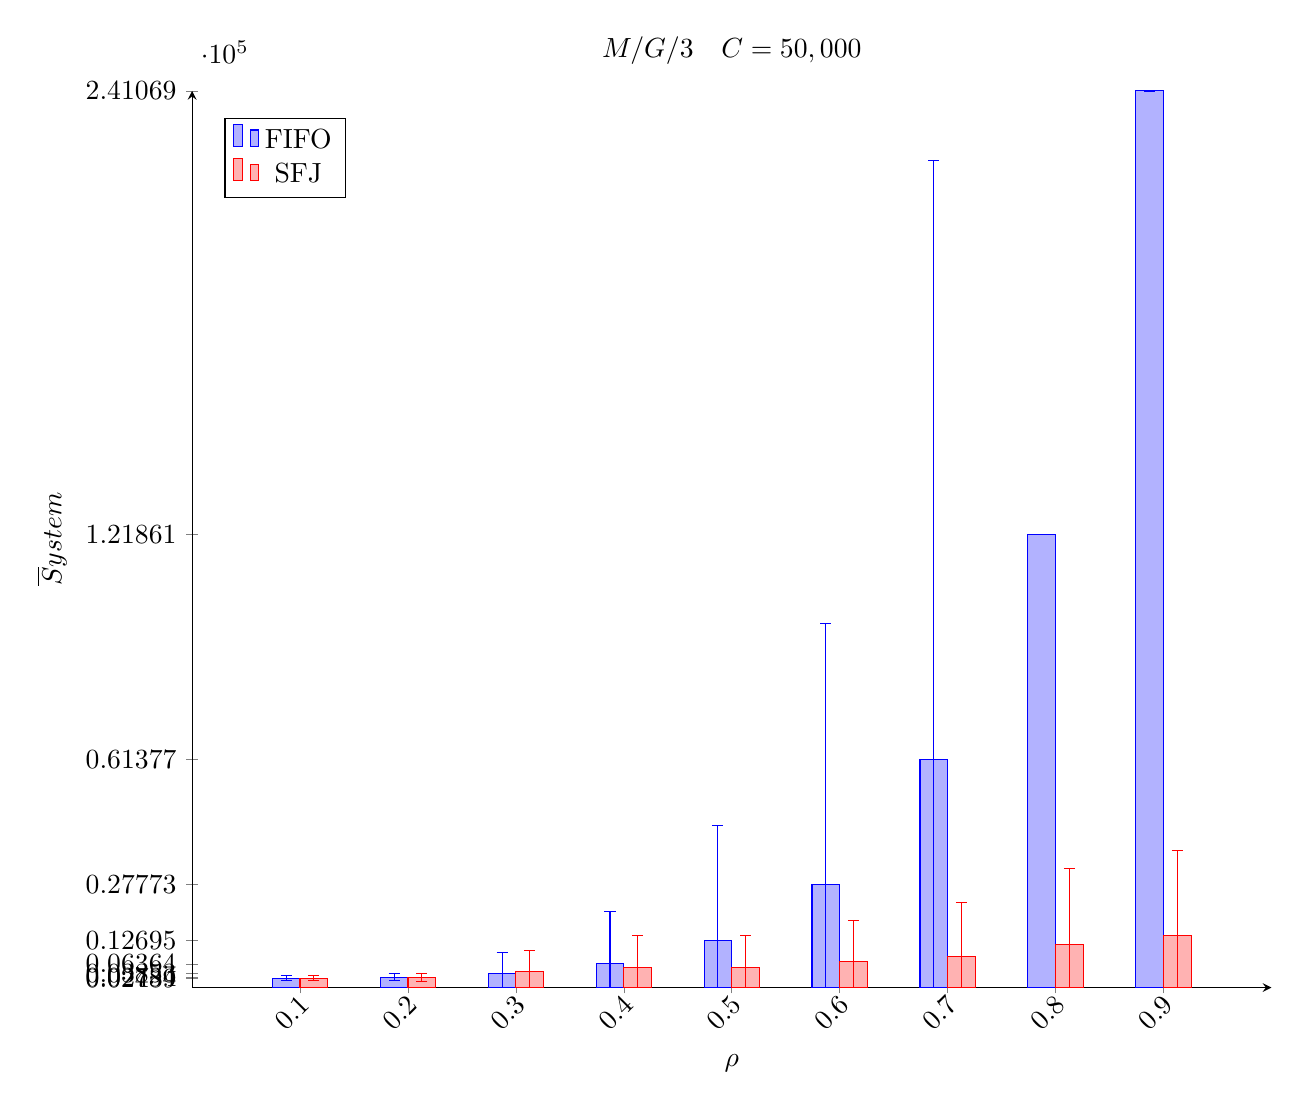
\begin{tikzpicture}[scale=1.0]
\begin{axis}[
    legend pos=north west,
    title= {$M/G/3 \quad C=50,000$},  
	ymin=0,
	y post scale=2,
	x post scale=2,
	ybar=0pt,
	enlargelimits={abs=0.5},
    xmin=0,
    xmax=1,
	xlabel = {$\rho$},
    ylabel = {$\overline{S}ystem$},
	xtick=data,
	ytick=data,
	ticklabel style={
        /pgf/number format/fixed,
        /pgf/number format/precision=5
	},
	x tick label style={rotate=45, anchor=east, align=center, xshift=.1cm,yshift=-0.1cm},
	axis lines=left
	]
\addplot+[error bars/.cd,
y dir=both,y explicit]
coordinates {
    (.1, 2489) +- (0.0, 666)
    (.2, 2734) +- (0.0, 945)
    (.3, 3853) +- (0.0, 5675)
    (.4, 6364) +- (0.0, 14067)
    (.5, 12695) +- (0.0, 30780)
    (.6, 27773) +- (0.0, 70129)
    (.7,61377) +- (0.0, 160917)
    (.8,121861) +- (0.0, 0)
    (.9,241069) +- (0.0, 0)};
\addplot+[error bars/.cd,
y dir=both,y explicit]
coordinates {
    (.1,2489) +- (0.0, 665)
    (.2,2662) +- (0.0, 1091)
    (.3,4208) +- (0.0, 5738)
    (.4,5509) +- (0.0, 8418)
    (.5,5509) +- (0.0, 8418)
    (.6,7077) +- (0.0, 10963)
    (.7,8413) +- (0.0, 14417)
    (.8,11469) +- (0.0, 20507)
    (.9,13969) +- (0.0, 22999)};
\legend{FIFO, SFJ}
\end{axis}
\end{tikzpicture}
\\
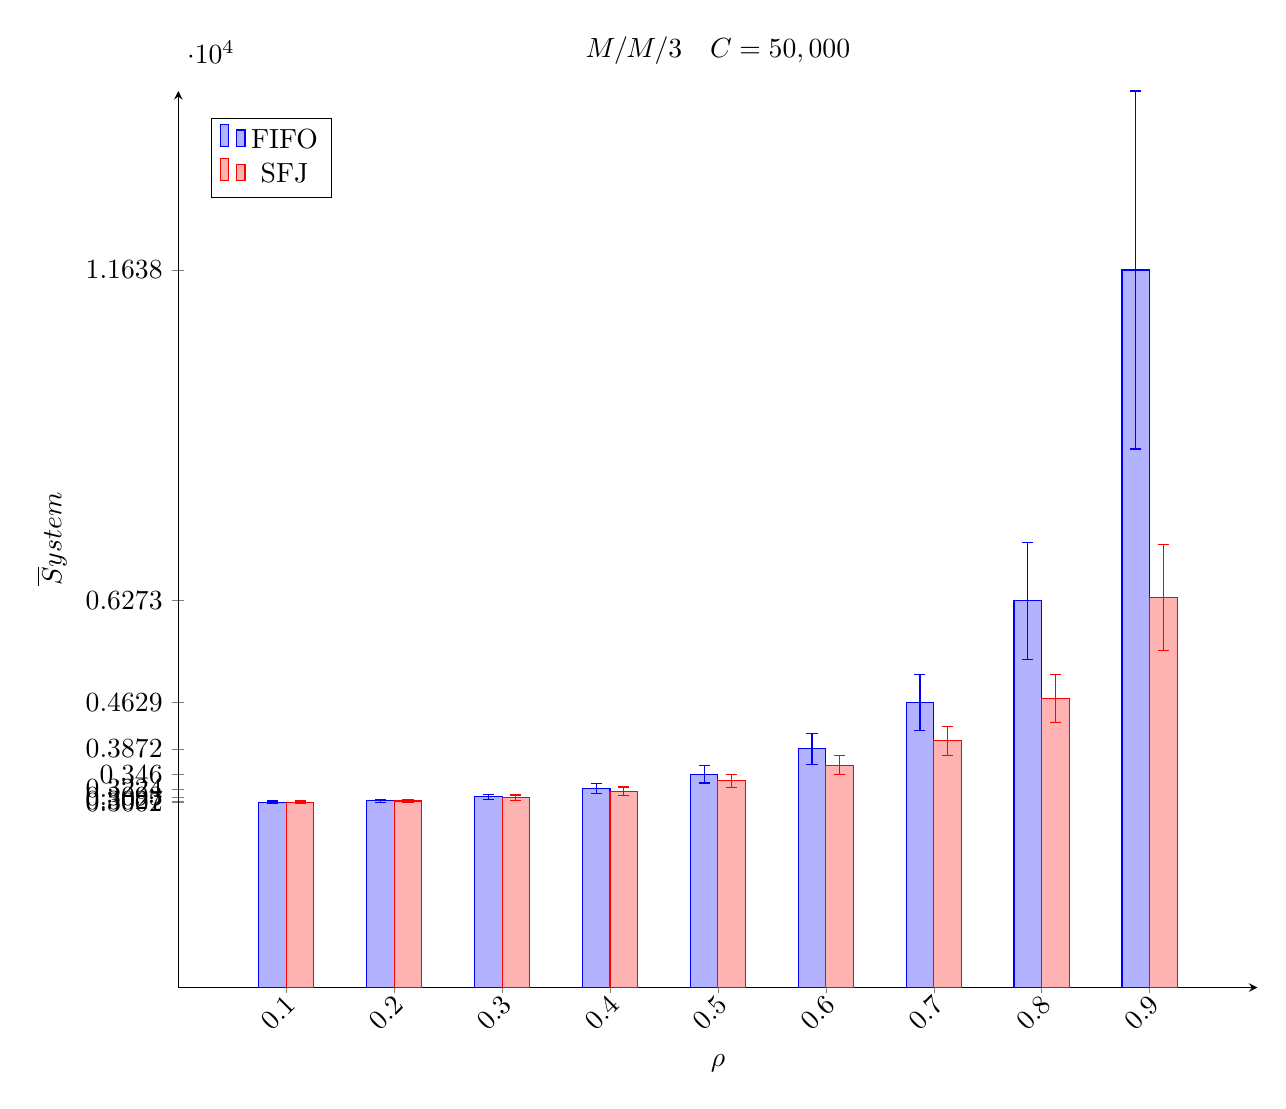
\begin{tikzpicture}[scale=1.0]
\begin{axis}[
    legend pos=north west,
    title= {$M/M/3 \quad C=50,000$},  
	ymin=0,
	y post scale=2,
	x post scale=2,
	ybar=0pt,
	enlargelimits={abs=0.5},
    xmin=0,
    xmax=1,
	xlabel = {$\rho$},
    ylabel = {$\overline{S}ystem$},
	xtick=data,
	ytick=data,
	ticklabel style={
        /pgf/number format/fixed,
        /pgf/number format/precision=5
	},
	x tick label style={rotate=45, anchor=east, align=center, xshift=.1cm,yshift=-0.1cm},
	axis lines=left
	]
\addplot+[error bars/.cd,
y dir=both,y explicit]
coordinates {
    (.1, 3002) +- (0.0, 23)
    (.2, 3027) +- (0.0, 28)
    (.3, 3093) +- (0.0, 45)
    (.4, 3224) +- (0.0, 81)
    (.5, 3460) +- (0.0, 142)
    (.6, 3872) +- (0.0, 249)
    (.7,4629) +- (0.0, 454)
    (.8, 6273) +- (0.0, 950)
    (.9, 11638) +- (0.0, 2903)
    };
\addplot+[error bars/.cd,
y dir=both,y explicit]
coordinates {
    (.1,3002) +- (0.0, 23)
    (.2,3025) +- (0.0, 27)
    (.3,3082) +- (0.0, 41)
    (.4,3185) +- (0.0, 67)
    (.5,3351) +- (0.0, 103)
    (.6,3605) +- (0.0, 155)
    (.7,4001) +- (0.0, 237)
    (.8,4689) +- (0.0, 394)
    (.9,6321) +- (0.0, 860)
    };
\legend{FIFO, SFJ}
\end{axis}
\end{tikzpicture}
\\
Note on graphing: error bars are omitted on the last two M/G/3 FIFO datapoints for readability.
\medskip
The variability of the Pareto distribution results in high variability, and the results are in line with expectation. The SJF discipline reduces overall system time by prioritizing shorter jobs, and this is especially true with long-tailed distributions where a large number of jobs will be starved due to high service times.
}
\bigskip
\newpage



%%%%%%%%%%%%%%%%%%%%%%
%%%%%%%%%%%%%%%%%%%%%%
%%%%%%%%%%%%%%%%%%%%%%

\textbf{Task 4}
This task involves the single-server queueing system. You will assume that $\rho = 0.5$ and that
$C = 100, 000$. Let $T(x)$ denote the total system time for a customer whose service time is $x$, and $W(x) =
T(x)-x$ its waiting time. We define the slowdown for a customer with service time $x$ as $S(x) = \frac{W(x)}{x}$. The slowdown can be thought of as a measure of fairness. The objective of this task is to see how the size of the service time affects the slowdown of the customer. For this, you need to compute the slowdown for each
of the $C$ customers, and for each of the two service disciplines (FCFS and SJF). Since there are too many
values of $S(x)$, making it difficult to plot, you will plot the slowdown against the percentile of the service
time distribution. Use $B = 100$ bins, and place each customer to the appropriate bin according to its service
time (i.e., the 1\% of customers with the smallest service times go into the first bin, the 1\% of customers with
the next smallest service times go to the second bin, etc). For each bin, take an average of the slowdown for
the customers in that bin. Then, plot the slowdown against the number of bins; compile two plots, one for
FCFS and one for SJF. What can you say about the fairness of each of these service disciplines? How do
the results compare to the slowdown of the processor sharing discipline which we discussed in class?\\
\\
\newcommand{\errorband}[5][]{ % x column, y column, error column, optional argument for setting style of the area plot
\pgfplotstableread[col sep=comma, skip first n=2]{#2}\datatable
    % Lower bound (invisible plot)
    \addplot [draw=none, stack plots=y, forget plot] table [
        x={#3},
        y expr=\thisrow{#4}-\thisrow{#5}
    ] {\datatable};

    % Stack twice the error, draw as area plot
    \addplot [draw=none, fill=gray!40, stack plots=y, area legend, #1] table [
        x={#3},
        y expr=2*\thisrow{#5}
    ] {\datatable} \closedcycle;

    % Reset stack using invisible plot
    \addplot [forget plot, stack plots=y,draw=none] table [x={#3}, y expr=-(\thisrow{#4}+\thisrow{#5})] {\datatable};
}
\medskip\\\texttt{
\\
\begin{tikzpicture}[scale=1.0]
\begin{axis}[
    legend pos=north west,
    title= {$M/G/3 \quad C=100,000$},  
	ymin=0,
	y post scale=2,
	x post scale=2,
	enlargelimits={abs=0.5},
    xmin=0,
	xlabel = {$\rho$},
    ylabel = {$Wait \%tile$},
	ticklabel style={
        /pgf/number format/fixed,
        /pgf/number format/precision=9
	},
	x tick label style={rotate=45, anchor=east, align=center, xshift=.1cm,yshift=-0.1cm},
	axis lines=left
	]
%\addplot +[mark=none] table [x=percent, y=mgmfifomean, col sep=comma]  {p4.csv};
%\addplot +[mark=none]  table [x=percent, y=mgmsjfmean, col sep=comma] {p4.csv};
\errorband[blue, opacity=0.5]{p4.csv}{0}{1}{2}
\errorband[red, opacity=0.5]{p4.csv}{0}{3}{4}
\legend{FIFO, SFJ}
\end{axis}
\end{tikzpicture}
\\
\begin{tikzpicture}[scale=1.0]
\begin{axis}[
    legend pos=north west,
    title= {$M/M/3 \quad C=100,000$},  
	ymin=0,
	y post scale=2,
	x post scale=2,
	enlargelimits={abs=0.5},
    xmin=0,
	xlabel = {$\rho$},
    ylabel = {$Wait \%tile$},
	ticklabel style={
        /pgf/number format/fixed,
        /pgf/number format/precision=9
	},
	x tick label style={rotate=45, anchor=east, align=center, xshift=.1cm,yshift=-0.1cm},
	axis lines=left
	]
%\addplot +[mark=none] table [x=percent, y=mmmfifomean, col sep=comma]  {p4.csv};
%\addplot +[mark=none]  table [x=percent, y=mmmsjfmean, col sep=comma] {p4.csv};
\errorband[blue, opacity=0.5]{p4.csv}{0}{5}{6}
\errorband[red, opacity=0.5]{p4.csv}{0}{7}{8}
\legend{FIFO, SFJ}
\end{axis}
\end{tikzpicture}
\\
Note on implementation and graphing: Error bands shown in shaded region. The work in queue at time the simulation finishes is not included in metrics. For SJF, this work in queue would - by definition - have the longest wait times.
\medskip
The FIFO discipline is inherently fair given random I.I.D. arrival and service times. The bounded pareto service distribution gives a very jagged percentile graph with high variance due to the outliers, but M/M/1 shows a completely level distribution.
\medskip
SFJ shows very low service times for all but most unfortunate, and the customers in the queue at the time of simulation end would be the most unfortunate of all.
\medskip
Why fairness? Fairness describes the concept of rough equal shared resource usage, and high slowdown reflects that sharing is not equal.}
\bigskip
\newpage


%%%%%%%%%%%%%%%%%%%%%%
%%%%%%%%%%%%%%%%%%%%%%
%%%%%%%%%%%%%%%%%%%%%%


\bigskip


\label{last}
\end{document}

